\section{Introduction}
\label{sec:intro}

\subsection{Modau River}

The Modau River is a small river located in the state of Hesse, Germany. Geographically, it originates in the Odenwald hills near Neunkirchen and flows northwest through a series of valleys and lowlands. The river stretches approximately 44 kilometres before it empties into the Rhine River near Stockstadt am Rhine. As it flows through town like Ober-Ramstadt, Pfungstadt, and parts of Darmstadt, the Modau shapes the surrounding landscape by contributing to the local drainage system and influencing soil fertility. Its drainage basin lies within a temperate climate zone, and the river plays a role in regional hydrology, especially in terms of groundwater surface-water runoff.

\begin{figure}[H]
	\centering
	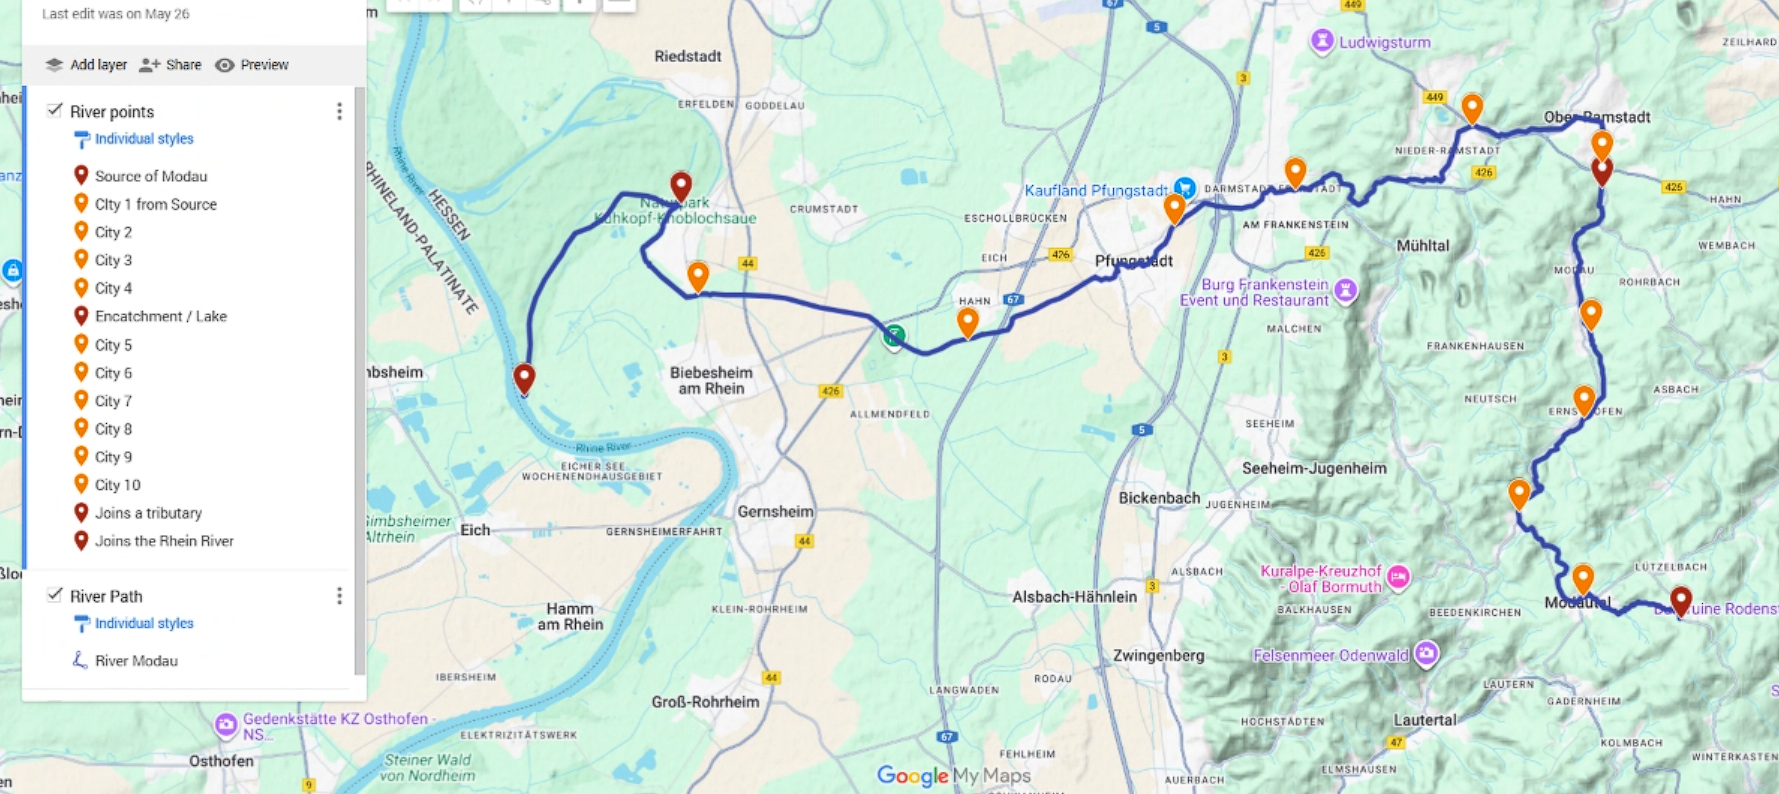
\includegraphics[width=0.9\textwidth]{Images/Selfmade_map_Modau.png}
	\caption{Map of Modau and towns and cities located on/near it using \textcite{googlemaps_darmstadt}.}
\end{figure}

As shown in the map, one can clearly follow the tributary from its source in the hills to the east, its upper course till Ober-Ramstadt where the river path is straight and in a v-shape valley, its middle course till Pfungstadt where it has entered its flat-floored valley leaving behind the hills with slight meanders which are more prominent when zoomed, and finally, the lower course as it joins the Rhine River. Here it is clearly a flat valley as the beige colour represents the surrounding farmland by the river. Meanders are clearer and more visible. As it flows to the River Rhine, the Modau has tributaries that flow into it the more we descend in altitude.

\subsection{Bradshaw Model}

\begin{figure}[H]
	\centering
	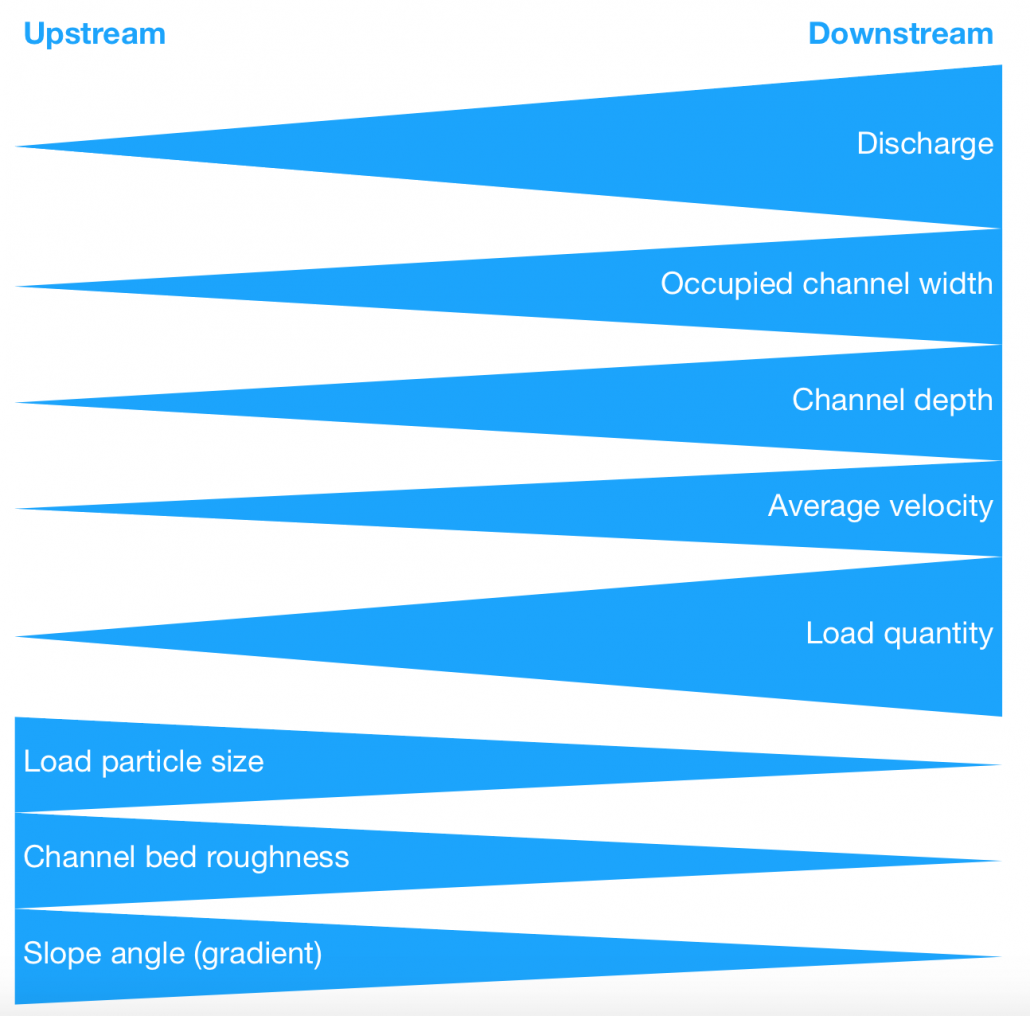
\includegraphics[width=0.65\textwidth]{Images/Bradshaw_Model.png}
	\caption{\textcite{internetgeography_riverfieldwork}}
\end{figure}

The Bradshaw Model is a geographical model which theorizes the characteristics of a river, stream, or tributary as one moves downstream from the source to the mouth \parencite{enacademic_weir}. However, the model can be read from both ways, upstream and downstream. Here it portrays how river discharge, channel width, depth, average velocity, and load quantity increase as one proceeds downstream. On the other hand, moving down stream, the load particle size, channel bed roughness, and gradient decrease \parencite{coolgeography_channelcharacteristics}. Despite showing the predicted river characteristics moving downstream, the Bradshaw Model does not encompass all the features of the river. Properties such as channel efficiency, river valley shapes and river landforms are exempt from this paradigm.

\subsection{Aim}

The aim of this following investigation is to determine the accuracy of the Bradshaw Model in predicting the characteristics of a river as it flows from its source down to its mouth.

\section{Hypotheses}
\label{sec:hypotheses}

\vspace*{0.5cm}


\begin{enumerate}
	\item As you move downstream, the velocity increases as channel efficiency increases. 
	\item As one moves downstream there is an increase in channel width and channel depth, the river discharge also increases.     
	\item Bedload size will decrease as we go downstream.
\end{enumerate}

